\chapter{Recherche du meilleur vaisseau}
	
Un vaisseau est considéré comme bon lorsqu'il gagne plus de combats que ses concurrents. 
On voit donc une logique évolutive où l'on compare tout le temps les vaisseaux entre eux et où l'on peut s'inspirer des meilleurs pour essayer de créer d'encore meilleurs vaisseaux. \\
Pour cela, il nous a tout d'abord fallu un générateur de vaisseaux. À partir de ce générateur nous avons pu utiliser un algorithme génétique qui permet d'avoir cette logique évolutive. 
Pour compléter l'optimisation des meilleurs vaisseaux, nous avons utilisé un système expert qui puise ses connaissances dans une base de données où sont stockées les différentes caractéristiques d'un groupe de vaisseaux.


	\section{Algorithmes de génération de vaisseaux}

	Un générateur doit créer un vaisseau en fonction d'un certain coût car c'est ce critère qui sépare les vaisseaux en différentes catégories. Tout d'abord, un générateur aléatoire est nécessaire pour parcourir tout les combinaisons d'équipement possibles. Ensuite, on veut un algorithme plus intelligent qui puisse parcourir ces combinaisons aléatoires pour tirer les meilleures et éventuellement les affiner.

		\subsection{Générateur aléatoire}
		
		\begin{figure}[H]
			\caption{Générateur aléatoire}
			\label{fig:randGen}
			\centering
			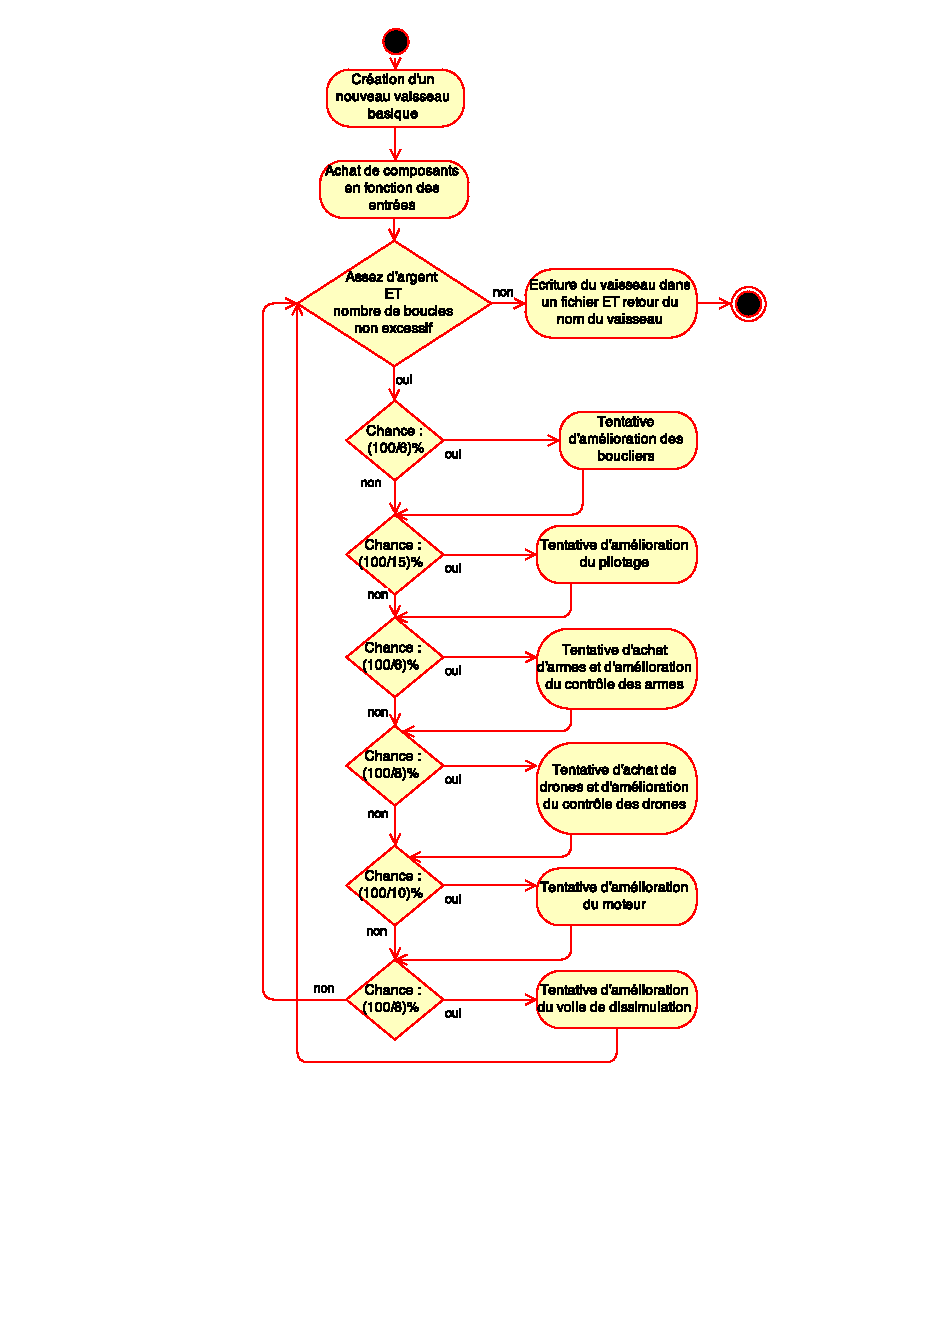
\includegraphics[width=0.65\linewidth]{randomGenerator.pdf}
		\end{figure}

		Le générateur aléatoire est simple puisque tant qu'il a de l'argent, il va essayer d'acheter quelque chose de façon aléatoire. Suivant les fonctionnalités gérées par le moteur de combat, nous avons construit le générateur aléatoire selon le schéma de la figure~\ref{fig:randGen}.

		On remarque que l'aléatoire est relativement guidé car certains équipements sont plus ou moins utiles et donc il y a plus ou moins de chance de les acheter. Ce choix a été fait pour éviter de tomber sur le moins de vaisseaux inutiles. Le fait d'avoir une boucle pour essayer chaque type d'équipement plutôt que de piocher à chaque fois un type d'équipement dans une liste est là pour éviter d'acheter des équipements différents pour créer des synergies. Dans les chances de choisir un type d'équipement il a fallu tenir compte des chances de tomber sur les équipements précédents.
		
		Les détails d'un achat potentiel dépendent en partie de l'équipement choisi. De façon générale pour un système, le générateur va d'abord calculer combien d'améliorations il peut acheter, puis acheter un nombre aléatoire d'améliorations. Directement après, il va essayer d'acheter un nombre aléatoire (inférieur ou égal à l'achat précédent) d'énergie. Prenons l'exemple des moteurs.
		
		\begin{figure}[H]
			\caption{Exemple des moteurs dans le générateur aléatoire}
			\label{fig:randGenEx}
			\centering
			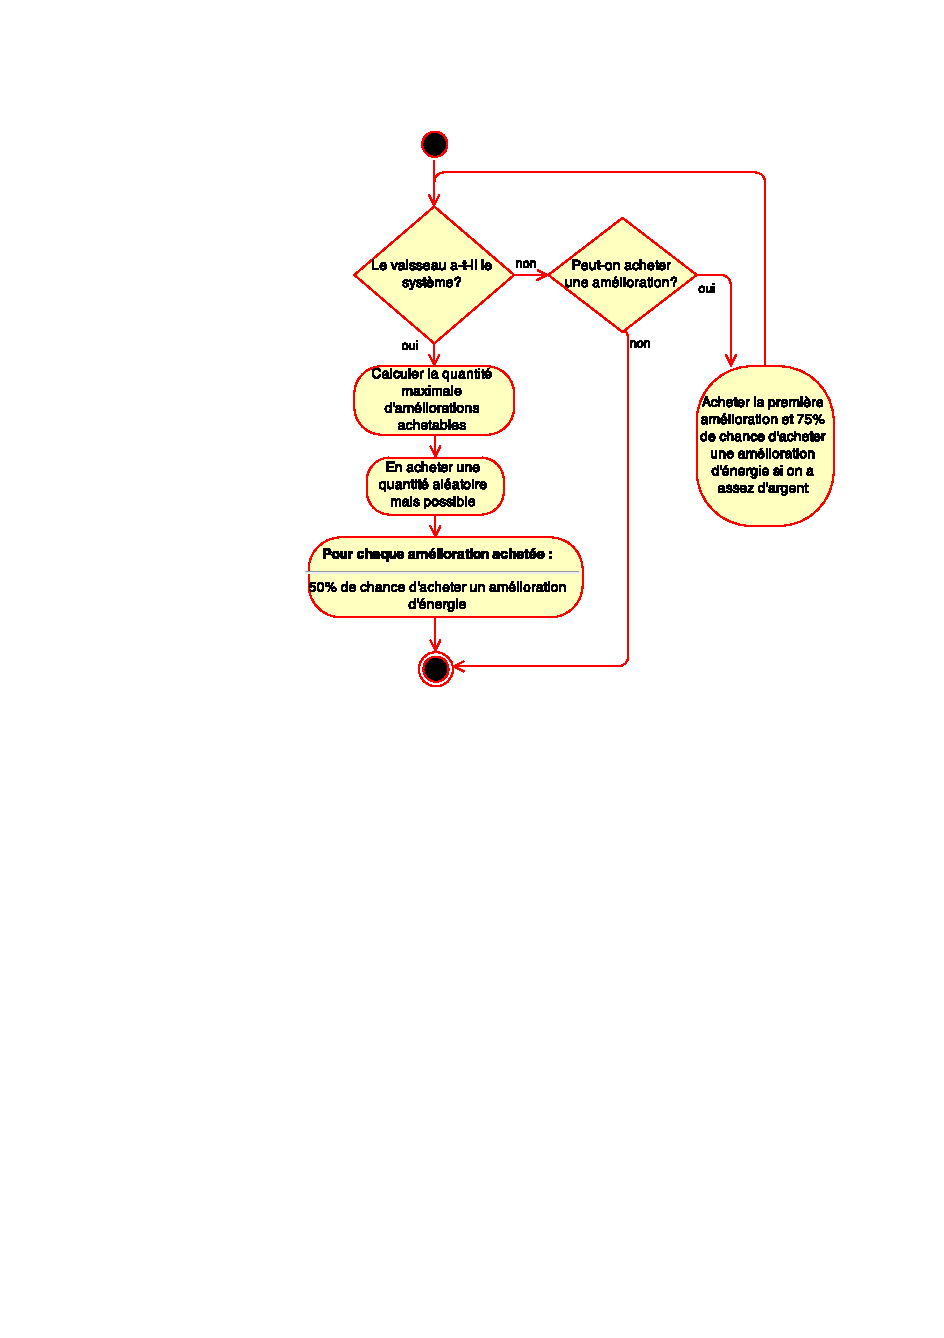
\includegraphics[width=0.65\linewidth]{randomGeneratorExample.pdf}
		\end{figure}

		Parmi les petits détails dépendant de l'équipement choisi, on peut citer :
		\begin{itemize}
			\item pour les boucliers le générateur va essayer d'acheter les améliorations par 2 mais avec une petite chance de n'acheter qu'une seule amélioration pour atteindre un palier pour pouvoir créer un \textit{buffer} ;
			\item pour le système des armes et celui des drones, le générateur choisit une arme (ou drone) aléatoirement, regarde s'il y a assez de place, regarde s'il y a assez d'argent, regarde le coût d'améliorations pour pouvoir alimenter toutes les armes et achète l'arme si toutes les conditions sont remplies, ensuite il achète un nombre aléatoire (plus petit ou égal à l'alimentation de l'arme choisie) d'énergie.
		\end{itemize}
		
		
		\subsection{Algorithme génétique}
		
		Un algorithme génétique reproduit l'évolution naturelle. On part donc d'une population et on détermine les individus qui sont les meilleurs (ceux qui survivraient dans la nature). À partir de ces individus, on crée une nouvelle population dont les individus peuvent avoir des mutations. On reproduit ainsi ce processus autant de fois que l'on veut.\\
		Dans notre cas, les individus sont des vaisseaux et les gènes sont les achats effectués. L'intégration de l'algorithme ressemble donc à cela.

		\begin{figure}[H]
			\caption{Algorithme génétique}
			\label{fig:genA}
			\centering
			\includegraphics[width=1\linewidth]{geneticalgorithm.pdf}
		\end{figure}
		
		Pour déterminer les meilleurs vaisseaux, on fait simplement un tournoi et on garde ceux qui ont gagné le plus de combats. Un tournoi consiste à faire combattre chaque vaisseau contre chacun des autres vaisseaux (on construit la partie supérieure à la diagonale d'un tableau carré). Un combat de tournoi (un match) est fait de plusieurs combats du moteur de combats et le gagnant est celui qui a gagné plus de la moitié des combats. \\
		Pour faire les croisements il faut deux vaisseaux issus des champions. Pour chacun de ces vaisseaux on garde en mémoire le nombre d'énergie acheté, les armes et drones achetés et les améliorations des systèmes. Ensuite, on crée un nouveau vaisseau de race et type identiques à un des deux vaisseaux pères. À partir de ce moment, on pioche aléatoirement dans les achats des parents pour les ajouter au nouveau vaisseau s'il a assez d'argent. \\
		Une mutation est tout simplement le vaisseau résultant d'un croisement entre un vaisseau existant et un nouveau vaisseau aléatoire. Les vaisseaux existants pris ne sont pas les champions de la génération précédente pour garder ces derniers et ne pas baisser dans la qualité des champions.
		
		L'algorithme s'arrête lorsqu'il y a eu trop de générations ou s'il y a une stabilisation chez les individus. Il y a stabilisation lorsqu'il n'y a plus de vaisseau vraiment plus fort que les autres, c'est-à-dire que tous les vaisseaux ont environ le même ratio de victoires.

		Au final, nous pouvons faire une étude (simple) de complexité de temps dans le pire des cas. Les tournois prennent la quasi-totalité du temps et pour faire les multiples combats des matchs, ils utilisent tous les processeurs disponibles. Il suffit donc de multiplier le nombre maximal de générations par le nombre de matchs dans un tournoi par le nombre de combats par match et par le temps moyen d'un combat et divisé par le nombre de processeurs de la machine. Si on prend \textit{g} le nombre de générations, \textit{n} le nombre de vaisseaux dans une population, \textit{c} le nombre de combats par match, \textit{t} le temps d'un combat et \textit{p} le nombre de processeurs, on obtient la formule suivante. \[\frac{gn(n-1)ct}{2p}\] Un algorithme typique et rigoureux aura $g:=30$ ; $n:=20$ ; $c:=21$ ; $t:=2$ secondes et $p:=4$. L'algorithme durera donc au maximum un peu plus de 16 heures.

	
	\section{Data Mining}
	
	Pour les parties de data mining nous avons utilisé le programme \textit{Linear time Closed itemset Miner} de Takeaki Uno qui nous permet d'extraire les caractéristiques (listes des équipements d'un vaisseau) les plus courantes dans une liste de vaisseaux.

	Ce programme prend en entrée un fichier où chaque ligne contient des entiers séparés par des espaces, chacune de ces lignes représente un ensemble d'entiers. 
	Le programme retourne ensuite tous les sous-ensembles de chaque ligne et donne le nombre d'occurrences de ces sous-ensembles dans toutes les lignes. La fouille fermée permet de ne garder que les ensembles qui ne sont pas des sous-ensembles d'autres lignes. On peut ensuite décider de ne garder que les sous-ensembles qui apparaissent dans au moins n lignes.\\
	
	Le fichier que l'on donne au programme LCM a une ligne pour chaque vaisseau et chaque ligne est constituée des équipements achetés et présents de base (dans les équipements on compte les armes, drones, améliorations et l'énergie). Pour utiliser ce programme il nous a donc fallu traduire les caractéristiques des vaisseaux en entiers, ce que nous avons fait de la façon suivante :
	\begin{itemize}
		\item pour l'énergie, on écrit simplement le nombre d'énergie disponible, donc un nombre compris entre 0 et 25 ;
		\item pour les améliorations des systèmes, on associe à chaque système un nombre plus grand que 3 et on concatène ce nombre avec le nombre d'améliorations faites (toujours moins que 9), le nombre final est compris entre 31 et 179 ;
		\item pour les armes, on associe à chaque arme un nombre et on concatène 10 avec ce nombre, le nombre final est compris entre 1001 et 1030 ;
		\item pour les drones, on associe à chaque drone un nombre et on concatène 11 avec ce nombre, le nombre final est compris entre 1101 et 1120.
	\end{itemize}
	À noter que dans le fichier d'entrée on écrit le niveau d'améliorations ou le niveau d'énergie avec les niveaux précédents pour avoir des sous-ensembles (e.g. pour un niveau de 3 d'énergie : energy1 energy2 energy3). \\

	Au final, le fichier résultat est un ensemble de listes d'équipements communs à plus ou moins de vaisseaux.
	
	
	
	\section{Déroulement de l'algorithme final d'optimisation}

	\begin{figure}[H]
		\caption{Algorithme final}
		\label{fig:finalG}
		\centering
		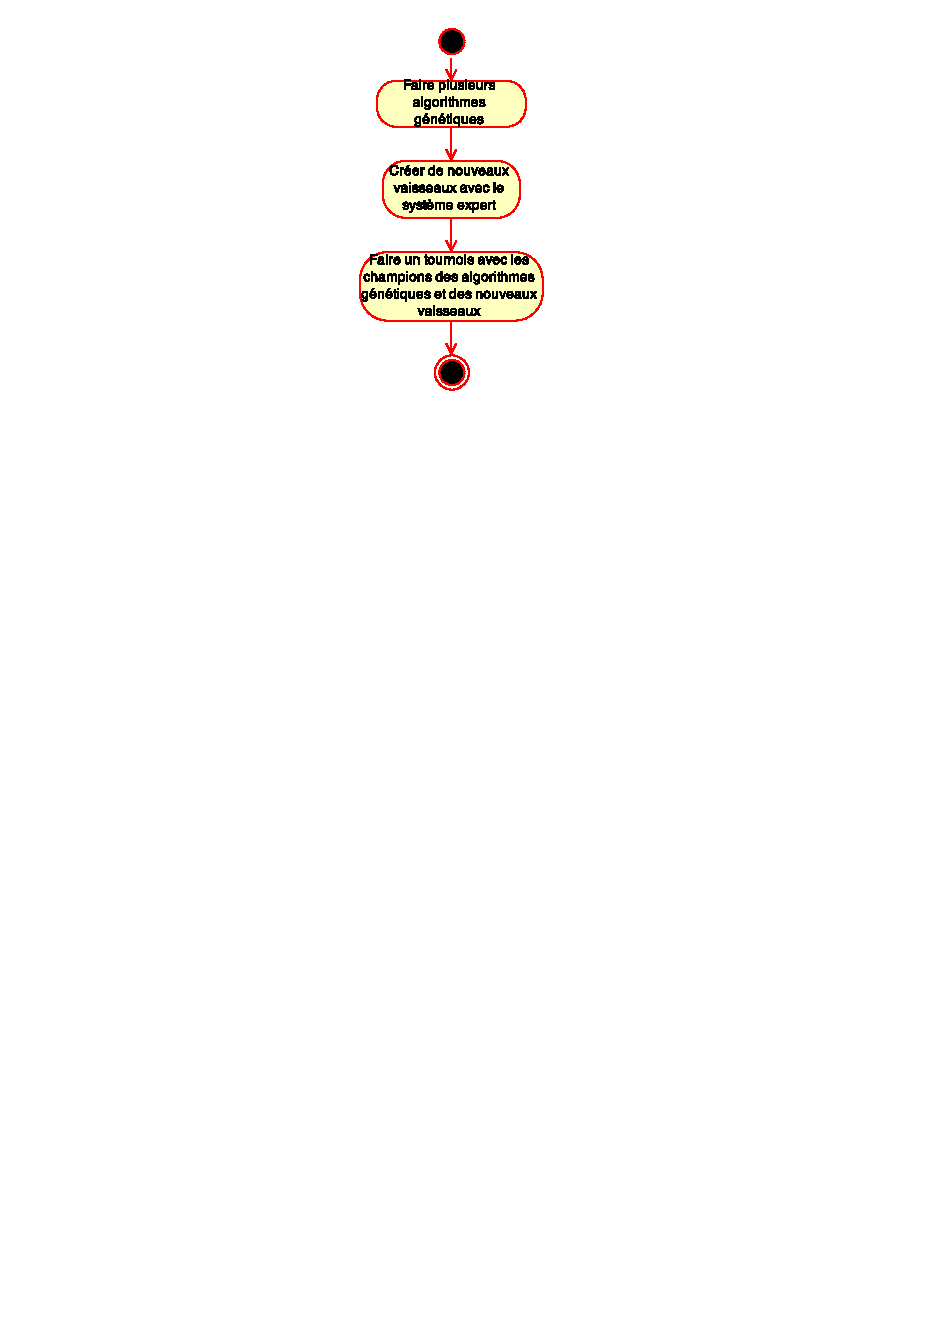
\includegraphics[width=0.34\linewidth]{finalAlgorithm.pdf}
	\end{figure}
	
	L'algorithme final (figure~\ref{fig:finalG}) est l'algorithme utilisé pour trouver le meilleur vaisseau. Pour cela il utilise des algorithmes génétiques et du \textit{data mining}. Au début il a plusieurs algorithmes génétiques distincts pour établir une base de vaisseaux avec des bons (les champions des algorithmes génétiques) et des mauvais vaisseaux. À partir de cette base de vaisseaux, on cherche les caractéristiques communes avec la technique de \textit{data mining} vu précédemment. Ensuite pour chaque caractéristique commune, on calcule le nombre d'occurrences chez les mauvais vaisseaux et aussi chez les bons vaisseaux. 

	Grâce à ces données on peut calculer le taux de croissance de chaque caractéristique commune avec la formule \[\mathlarger{\rho (P) = \frac{\ \ \mathlarger{\frac{S_{+}}{D_{+}}} \ \ }{\ \ \mathlarger{\frac{S_{-}}{D_{-}}} \ \ }} \] où $S_{\pm}$ est le nombre d'occurrences chez les bons/mauvais vaisseaux et $D_{\pm}$ est le nombre de bons/mauvais vaisseaux. Si le nombre d'occurrences chez les mauvais vaisseaux est nul alors le taux vaut \[\mathlarger{\rho (P) = \frac{\ \ \mathlarger{\frac{S_{+}}{D_{+}}} \ \ }{\ \ \mathlarger{\frac{1}{D_{-}^{2}}} \ \ }} \] Ce taux est toujours positif et si ce taux est plus grand que 1, alors la caractéristique est relativement plus commune chez les bons vaisseaux, donc est peut-être une caractéristique déterminante pour faire d'un vaisseau un bon vaisseau. Pour être vraiment sur d'une caractéristique déterminante, nous utilisons aussi un taux de confiance qui a pour formule \[\mathlarger{\mbox{conf} = \frac{\rho (P)}{\rho (P)+1}} \] Ce taux permet d'évaluer la grandeur du taux de croissance et donc évaluer la déterminance d'une caractéristique pour faire de bons vaisseaux.

	On obtient donc les caractéristiques déterminantes. Pour chacune de ces caractéristiques, un vaisseau de chaque race et de chaque type va être créé avec le générateur aléatoire auquel on aura donné la caractéristique à acheter en premier. Ensuite on ne garde que les vaisseaux qui ne semblent pas mauvais. Un vaisseau valide ce test si sa race, son type et ses équipements ne font pas partie des \textit{low tiers} de \textit{tiers lists} trouvées sur internet. À partir de cette liste de nouveaux vaisseaux et des vaisseaux gagnants des algorithmes génétiques, un tournoi est fait pour déterminer le meilleur d'entre eux et c'est celui-ci qui est retourné par l'algorithme au final.

	Le temps de cet algorithme est équivalent au temps mis par les algorithmes génétiques du début car le programme \textit{LCM} de data mining est très rapide.
